\documentclass{sciposter}
\usepackage{lipsum}
\usepackage{epsfig}
\usepackage{amsmath}

\usepackage{amssymb}
\usepackage{bm}
\usepackage{multicol}
\usepackage{graphicx,url}
\usepackage[english]{babel}   
\usepackage[utf8]{inputenc}
\usepackage{dsfont}
\newtheorem{Def}{Definition}


\title{Recursive CNNs for ImageToLatex problem}
%Título do projeto

\author{Michał Tyrolski, Szymon Tworkowski}
%nome dos autores

\institute 
{Student @ Faculty of Mathematics, Informatics and Mechanics - University of Warsaw}
%Nome e endereço da Instituição

\email{}

%\date is unused by the current \maketitle


% Exibe os logos (direita e esquerda) 
% Procure usar arquivos png ou jpg, e de preferencia mantenha na mesma pasta do .tex
%%%%%%%%%%%%%%%%%%%%%%%%%%%%%%%%%%%%%%%%%%%%%%%%%%%%%%%%%%%%%%%%%%%%%%%%%%%%%%%%
%%% Begin of Document



\begin{document}
%define conference poster is presented at (appears as footer)

\conference{{\bf ML in PL: Virtual Event 2020}, Poster expo}

%\LEFTSIDEfootlogo  
% Uncomment to put footer logo on left side, and 
% conference name on right side of footer

% Some examples of caption control (remove % to check result)

%\renewcommand{\algorithmname}{Algoritme} % for Dutch

%\renewcommand{\mastercapstartstyle}[1]{\textit{\textbf{#1}}}
%\renewcommand{\algcapstartstyle}[1]{\textsc{\textbf{#1}}}
%\renewcommand{\algcapbodystyle}{\bfseries}
%\renewcommand{\thealgorithm}{\Roman{algorithm}}

\maketitle

%%% Begin of Multicols-Enviroment
\begin{multicols}{3}

%%% Abstract
\begin{abstract}
While recurrent neural networks became the most accurate solution for the ImageToLatex problem, they are used along with lots of tricky architecture improvements. Commonly used approach is to connect CNN encoders with some RNN decoders with attention mechanisms attached. We show a more human-like approach based on tree structure analysis of expressions using divide-and-conquer algorithm. According to the fact that our approach tries to split expression in several parts, we also prepared a dataset with unambiguous expression splits, representing some LaTeX subset. We compared the  state-of-the-art model vs our structure model with that SOTA used for leaf recognition. Finally we show that our approach performed better on our dataset with a particular number of splits.


\end{abstract}

%%% Introduction
\section{Introduction}
ImageToLatex is quite an old problem. Before the deep learning era, it was commonly approached with different ideas related to optical character recognition (OCR) methods [1]. Recently using encoder + decoder architecture with modification became the most popular approach to produce latex expression from image. In such models, encoder often has convolutional neural networks (CNN) as a backbone for producing feature maps [2,3,4], sometimes using custom modifications like row-encoding [2]. For decoding, there are usually recurrent neural networks (RNN) [2,3,4]. 

In this work we modify the parsing expression idea presented by Zanibbi, R. and all [5]. Instead of old OCR methods, we use CNNs to predict bounding boxes for operators and operands. Recursively repeating cnn calls gives us knowledge about expression tree structure with bounding boxes for each expression subtree. Then any model can be used to recognize leafs, especially those with ability to properly recognize expressions with bounded length by a constant $C$ for example like stacked CNNs [6].

\section{Model}
\subsection{Structural Model $M_{\mathcal{S}}$}
Model responsible for building the tree structure is CNN with ResNext18 [10] as a backbone with a small custom head. Bounding boxes are predicted along with categories simultaneously. Category is represented as 1-hot encoding and each bounding box $(x_1,y_1,x_2,y_2)$ as $$(x_1,y_1,\sqrt{x_2-x_1},\sqrt{y_2-y_1})$$
Similarly to Redmon,  J. and others, we define loss function $\mathcal{L}$ for a batch as follows [9]:

$$
 \mathcal{L} (\{B_i\}, \{C_i\}) = \frac{1}{N} \sum_i \left( \mathcal{L}_1(C_i, C_i^*) +  \lambda \mathcal{H}(C_i^*) \mathcal{L}_2(B_i, B_i^*)  \right)
$$

where $\mathcal{L}_1 = \operatorname{LOGLOSS}$, $\mathcal{L}_2 = \operatorname{MSE}$ and $(B_i, B_i^*), (C_i, C_i^*)$ are predicted, ground-truth values for boxes and categories respectively, $\mathcal{H}(C)=\mathds{1}_{C \neq \text{leaf}}$. Purpose of $\lambda$ is to increase the effect of box loss and it is empirically chosen. In our case $\lambda = 50$. Accuracy of structural model is measured as pair $\mathcal{A}=(I, A_c)$ where $I=\operatorname{IOU}$ and $A_c$ is a standard accuracy. On our dataset we achieved $\mathcal{A}=(99.9\%,95.4\%)$ for the first split.

$M_{\mathcal{S}}$ proceed with recursive calls to CNN (Figure 1) as long as it doesn't detect a leaf or achieve a hyperparam depth limit but training is done only to first split for each entry from the dataset.

\begin{figure}[h]
\begin{center}
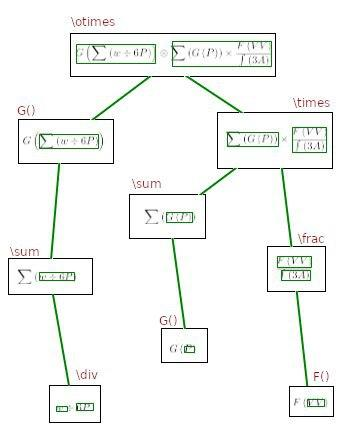
\includegraphics[width=16cm]{cnn.jpg}
\end{center}
\caption{ \label{fig:tree} Sample expression tree built with recursive calls to CNN. Own research.}
\end{figure}

During inference, each node which isn't recognized as a leaf is centered and appended with white rows and cols in order to match the input shape. Then the next CNN call is taken.

\subsection{Leaf Model $M_{\mathcal{L}}$}
As a recognizer for leafs and baseline to compare we chose Yuntian Deng, Anssi Kanervisto, Jeffrey Ling, Alexander M. Rush 2016: Image-to-Markup Generation with Coarse-to-Fine Attention. We trained that model for $15$ epochs on a full dataset. Expression depth $d$ is defined as the number of nodes in the longest path from root to leafs. If $M_{\mathcal{S}}$ stops before reaching $d$, $M_{\mathcal{L}}$ is used as a recognizer for the whole subtree.

\subsection{Dataset}
Dataset is generated from scratch. It contains $100008$ images with shape $(224,224,3)$. We support $17$ operators, $8$ of them unary, another $8$ binary and $1$ leaf. We decided to create our own dataset because $M_{\mathcal{S}}$ need bounding boxes coordinates. Each entry in the dataset consists of the following information: name, operator name, sorted operands bounding boxes in form of $(x,y,dx,dy)$, normalized label and depth. Max supported depth is $4$, deeper equations were unreadable in that resolution.

\begin{figure}[h]
\begin{center}
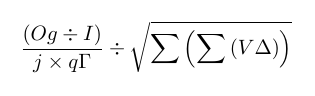
\includegraphics[width=10cm]{eq85004_b.png}
\end{center}
\begin{center}
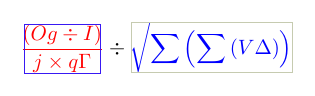
\includegraphics[width=10cm]{eq85004_c.png}
\end{center}
\caption{ \label{fig:eigen} Sample with depth $4$ along with labeled version.  Own research.}
\end{figure}

In order to generate a dataset, we had to create a $M_{\mathcal{S}}$ loss function to take into account various possible splits along with ensuring the convergence of the model or find an unambiguous way of splitting the expressions. We went with the second approach. The split is done on the left most inline operator if the operator on top is binary, otherwise the argument of unary operator is taken.

Let $E(d)$ be a set of all expression with depth $\le d$ and $\operatorname{In}: P(\operatorname{Expr}) \rightarrow P(\operatorname{Expr})$ such that
\nonumber
\begin{equation}
\begin{split}
\operatorname{In}(S) & = \{ e_1 \triangle e_2 | e_1 \text{ is not an inline expression} \} \\
& \cup  \{\Delta(e) | \Delta \text{ is an unary operator} \} \\
& \cup  \{\Delta(e_1,e_2) | \Delta \text{ is not an inline operator }\}
\end{split}
\end{equation}
In our case inline operators $\in \{+, \times, \star, \div, \otimes, -, \cdot \}$ and an expression is inline if and only if the top operator is inline. Also, notice that $\forall d$ there is a bijection between $\operatorname{In}\left(E(d)\right)$ and $E(d)$. That observation allowed us to generate a dataset without need to parse latex expressions. Instead of sampling from $E(d)$ and parsing them, we generated colorful $\operatorname{In}\left(E(d)\right)$ and deterministically detected boxes as shown in Figure 2. As part of augmentation, we decreased the quality of a small sample of dataset depending on sample depths in order to simulate an inference process.

\section{Results and discussions}

\subsection{Comparison}
We compared $M_{\mathcal{S}}$ with $M_{\mathcal{L}}$ for subtree recognizing versus $M_{\mathcal{L}}$ for whole sentence recognizing. Results are shown in Table 1.

\begin{table}[ht] 
\caption{Comparison between $M_{\mathcal{S}}$+$M_{\mathcal{L}}$ and $M_{\mathcal{L}}$.  Own research.} %title of the table 
\centering % centering table 
\begin{tabular}{c| rr  } % creating eight columns 
\hline\hline %inserting double-line 
Depth limit &BLEU&EDIT\\ [0.25ex] 
\hline   
0 Baseline & $81.1\%$ & $78.1\%$  \\  
1 $M_{\mathcal{S}}$+$M_{\mathcal{L}}$ & $\bm{89.1\%}$ & $\bm{85.4\%}$  \\
2 $M_{\mathcal{S}}$+$M_{\mathcal{L}}$ & $\bm{87.2\%}$ & $\bm{82.4\%}$  \\  
3 $M_{\mathcal{S}}$+$M_{\mathcal{L}}$ & $\bm{83.3\%}$ & $75.6\%$  \\  
4 $M_{\mathcal{S}}$+$M_{\mathcal{L}}$ & $80.3\%$ & $68.2\%$  \\  

\hline\hline  
\end{tabular} 
\label{tab:hresult} 
\end{table} 

As shown in table, $M_{\mathcal{S}}$+$M_{\mathcal{L}}$ achieves much better results for $1$ and $2$ depth steps and better BLEU metric for $d=3$. As can be expected, for more steps baseline still achieves better scores. We identify two main reasons for decreasing dominance of  $M_{\mathcal{S}}$+$M_{\mathcal{L}}$ over $M_{\mathcal{L}}$ standalone. Firstly, while $M_{\mathcal{S}}$ first bounding box detection is almost ideal, error propagates and at a certain depth model is not able to recognize proper boxes. Moreover, after each $M_{\mathcal{S}}$ inference, we rescale box expression which degrades the quality of next input images. Our augmentation mentioned in the dataset section improves $M_{\mathcal{S}}$ but after few rescaling expressions become unreadable, even for humans. On the other hand, many im2seq models have problems recognizing the structure of long expressions, especially without much training. It can be concluded that our approach has potential to improve accuracy using a small number of splits for sota models on real itl100k dataset.


\subsection{Future work}
That approach is able to improve many models on image to sequence problems. In order to compete on real dataset, current one should be extended for more symbols, more unary and binary operators along with operators with much more operands. Also upper and lower indexes and complex structures like matrices should be supported. It should be considered if it is worth to detect forest structure instead of trees only, especially if the target is to generalize. To make models useful on a bigger scale, architecture should accept bigger shapes, custom too. Also, in terms of longer sequences it is worth to think about loss and dataset creation which prefer the middle operator.

\section{Implementation}

To ensure the reproducibility of this work and to support open science principles, we made the code and dataset available on https://github.com/kakainet/TexNet and https://github.com/kakainet/TexSet. Details are provided in the readme. Code is written in fast.ai [7] and PyTorch [8]. We use ready implementation of model proposed by Deng, Y. and all [2], with small modifications related to data augmentation as a backbone and train on our dataset.
 
\section{References}

\begin{enumerate}

\item Suzuki, M., Kanahori, T., Ohtake, N. and Yamaguchi, K., 2004, July. An integrated OCR software for mathematical documents and its output with accessibility. In International Conference on Computers for Handicapped Persons (pp. 648-655). Springer, Berlin, Heidelberg.

\item Deng, Y., Kanervisto, A., Ling, J. and Rush, A.M., 2017, July. Image-to-markup generation with coarse-to-fine attention. In International Conference on Machine Learning (pp. 980-989).

\item Wang, J., Sun, Y. and Wang, S., 2019. Image to latex with densenet encoder and joint attention. Procedia computer science, 147, pp.374-380.

\item Genthial, G. and Sauvestre, R., 2016. Image to Latex.

\item Zanibbi, R., Blostein, D. and Cordy, J.R., 2002. Recognizing mathematical expressions using tree transformation. IEEE Transactions on pattern analysis and machine intelligence, 24(11), pp.1455-1467.

\item More, A., 2018. IMAGE TO LATEX VIA NEURAL NETWORKS.

\item Howard, J. and Gugger, S., 2020. Fastai: A layered API for deep learning. Information, 11(2), p.108.

\item Paszke, A., Gross, S., Massa, F., Lerer, A., Bradbury, J., Chanan, G., Killeen, T., Lin, Z., Gimelshein, N., Antiga, L. and Desmaison, A., 2019. Pytorch: An imperative style, high-performance deep learning library. In Advances in neural information processing systems (pp. 8026-8037).

\item Redmon, J., Divvala, S., Girshick, R. and Farhadi, A., 2016. You only look once: Unified, real-time object detection. In Proceedings of the IEEE conference on computer vision and pattern recognition (pp. 779-788)..

\item Xie, S., Girshick, R., Dollár, P., Tu, Z. and He, K., 2017. Aggregated residual transformations for deep neural networks. In Proceedings of the IEEE conference on computer vision and pattern recognition (pp. 1492-1500).

\end{enumerate}

%% Note: use of BibTeX als works!!

%\bibliographystyle{plain}
%\begin{thebibliography}{1}

%\bibitem{Flusser:Suk:93}
%J.~Flusser and T.~Suk.
%\newblock Pattern recognition by affine moment invariants.
%\newblock {\em Pattern Recognition}, 26:167--174, 1993.

%\bibitem{Hu:62}
%M.~K. Hu.
%\newblock Visual pattern recognition by moment invariants.
%\newblock {\em IRE Transactions on Information Theory}, IT-8:179--187, 1962.

%\bibitem{maragos89:_patter}
%P.~Maragos.
%%\newblock Pattern spectrum and multiscale shape representation.
%\newblock {\em IEEE Trans. Patt. Anal. Mach. Intell.}, 11:701--715, 1989.

%\bibitem{Meijster:Wilkinson:PAMI}
%A.~Meijster and M.~H.~F. Wilkinson.
%\newblock A comparison of algorithms for connected set openings and closings.
%\newblock {\em IEEE Trans. Patt. Anal. Mach. Intell.}, 24(4):484--494, 2002.

%\bibitem{Nacken:thesis}
%P.~F.~M. Nacken.
%\newblock {\em Image Analysis Methods Based on Hierarchies of Graphs and
%  Multi-Scale Mathematical Morphology}.
%\newblock PhD thesis, University of Amsterdam, Amsterdam, The Netherlands,
%  1994.

%\end{thebibliography}

\end{multicols}

\end{document}